\zerar
\chapter{Heurísticas}
\label{cap:heuristicas}

Os métodos exatos de solução do PDV resolvem, utilizando técnicas de otimização, o modelo de
programação linear inteiro (\ref{eq:sppv}). Dessa forma, uma solução ótima global para o problema é
obtida~\cite{anbil91b}. A resolução pelo otimizador é feita inicialmente considerando uma versão
relaxada do problema, \ie, permitindo que as variáveis $x_j$ assumam valores {\it reais} entre 0 e
1. A seguir, o problema relaxado é resolvido pelo método Simplex, ou alguma especialização do mesmo,
o que gera uma solução ótima fracionária $x^\ast$. A partir de $x^\ast$, empregando-se um esquema
{\it branch-and-bound}, ou {\it branch-and-cut}, obtém-se a melhor solução inteira. Vale ressaltar
que tais procedimentos de enumeração implícita consomem tempo e memória exponencial no número de
variáveis. Assim, a aplicação de tais métodos limita-se a instâncias pequenas.

Diversos métodos heurísticos foram desenvolvidos ao longo dos anos para lidar com o número
gigantesco de variáveis do problema e a incapacidade dos otimizadores lidarem com elas. Uma
listagem descritiva das principais heurísticas pode ser encontrado em~\cite{gopalakrishnan05}.

Após análise da literatura, resolvemos estudar mais a fundo e implementar três alternativas: um
método de busca local, um algoritmo genético híbrido e um procedimento de geração de colunas. 

Busca local foi a primeira heurística historicamente adotada pelas empresas para resolver seus
grandes problemas de escalonamento, levando a resultados satisfatórias~\cite{gershkoff89} na década
de 80. Dentre as meta-heurísticas, algoritmos genéticos vem sendo mais recentemente aplicados como
forma de se obter uma solução aproximada~\cite{kornilakis02}. Os resultados para problemas grandes,
entretanto, ainda não são satisfatórios. Finalmente, procedimentos de geração de colunas representam
o estado-da-arte dos métodos de solução, e constituem a base dos poderosos métodos do tipo {\it
branch-and-price}~\cite{vance97}.

%%%%%%%%%%%%%%%%%%%%%%%%%%%%%%%%%%%%%%%%%%%%%%%%%%%%%%%%%%%%%%%%%%%%%%%%%%%%%%%%%%%%%%%%%%%%%%%%%%%%

\section{Refatornado o Modelo}
\label{sec:refatorando}

Antes de explicarmos em mais detalhes cada uma das heurísticas estudadas, vamos fazer uma pequena
modificação ao modelo (\ref{eq:sppv}). Observe que o mesmo não admite a existência de {\it
deadheading}, \ie, tripulação viajando como passageiro. Em algumas situações isso pode implicar na
inviabilidade do problema.

A formulação que adotaremos a seguir modela o problema conhecido por {\it set cover}. Ele é bastante
similar ao {\it set partition}, porém admite a ocorrência de {\it deadheading} na solução final,
tornando possível a existência de soluções viáveis para o problema original.

As restrições no {\it set cover} são dadas pelas equações (\ref{eq:dh}), onde permite-se que 
uma etapa seja coberta mais do que uma vez. Sendo $m$ o número de etapas a serem cobertas, podemos 
adicionar $m$ variáveis artificiais inteiras $y_i$, $i = 1, \ldots, m$, onde $y_i$ representa o 
número de vezes que a etapa $i$ é coberta como {\it deadhead}. Considerando um custo $d_i$ cada vez 
que a etapa $i$ é utilizada como {\it deadhead}, o problema de programação linear resultante é
%
\begin{eqnarray} \label{eq:scpdv}
	\text{minimizar} && \displaystyle \sum_{j=1}^n c_j x_j + \sum_{i=1}^m d_i y_i \nonumber \\
	\text{sujeito à} && \displaystyle \sum_{j=1}^n a_{ij} x_j - y_i = 1 \ev \;\; i = 1, \ldots, m \\
	                 && x_j \in \{0, 1\} \ev \;\; j = 1, \ldots, n \nonumber \\
	                 && y_i \geq 0 \ev \;\; i = 1, \ldots, m \ep \nonumber
\end{eqnarray}

A adoção de custos altos associados às varáveis $y_i$ faz com que elas sejam naturalmente expulsas 
da base no final, levando a uma solução livre de {\it deadheading}, se alguma existir. Isso funciona
mais ou menos como o método-$M$ na primeira fase do algoritmo Simplex para obtenção de uma solução 
viável básica.

A vantagem do modelo (\ref{eq:scpdv}) é que com ele fica mais fácil encontrar uma solução viável
inicial para o problema. Como é permitido a sobreposição de etapas, podemos ir percorrendo a rede
de voos e ir gerando as viagens. Toda vez que uma nova viagem gerada cobrir uma perna não coberta,
armazenamos essa viagem na solução. Paramos quando todas as pernas tiverem sido cobertas.

%%%%%%%%%%%%%%%%%%%%%%%%%%%%%%%%%%%%%%%%%%%%%%%%%%%%%%%%%%%%%%%%%%%%%%%%%%%%%%%%%%%%%%%%%%%%%%%%%%%%

\section{Busca Local}
\label{sec:metodos_busca}

Busca local é uma abordagem geral utilizada para encontrar soluções de boa qualidade para problemas
de otimização combinatória difíceis, em tempo aceitável. O método é baseado em uma exploração 
iterativa de vizinhos da solução tentando melhorar a solução atual através de alterações locais.

A solução encontrada por um algoritmo de busca local tem a garantia apenas de ser ótima com relação
a alterações locais e, em geral, não será a solução ótima global.

O método de busca local no contexto do PDV é bastante simples e foi um dos primeiros a ser utilizado
na tentativa de melhorar uma solução viável do problema (\ref{eq:scpdv}). Basicamente o método
consiste em escolher aleatoriamente um número pequeno $k$ de viagens da solução viável inicial
(subproblema) e, a partir da lista de etapas cobertas e tripuladas por essas viagens, gerar
explicitamente todas as possíveis viagens legais usando o gerador. Como o número de etapas não é
muito grande, o número de variáveis geradas é gerenciável. O modelo (\ref{eq:scpdv}) é então
resolvido pelo otimizador para todas essas variáveis, obtendo-se um novo conjunto de viagens que
cobre o lista inicial de etapas. Se o custo desse novo conjunto de viagens for menor do que o
original, então as viagens originais serão substituídas na solução inicial. O processo é iterado um
número máximo de vezes (ou um tempo máximo de execução), ou até que não haja variação significativa
do custo (mínimo local), de tal forma que o custo sempre seja reduzido a cada passo.

Um fluxograma da execução do algoritmo é apresentado na Figura~\ref{fig:busca_local}. Note que se
tivermos uma boa rotina de geração de viagens e otimização, o método pode ser facilmente 
implementado. O sucesso na aplicação do método depende crucialmente do fato de sermos capazes de 
resolver eficientemente o PLI (\ref{eq:scpdv}) para um número pequeno de variáveis.

\begin{figure}[htbp]
	\begin{center}
		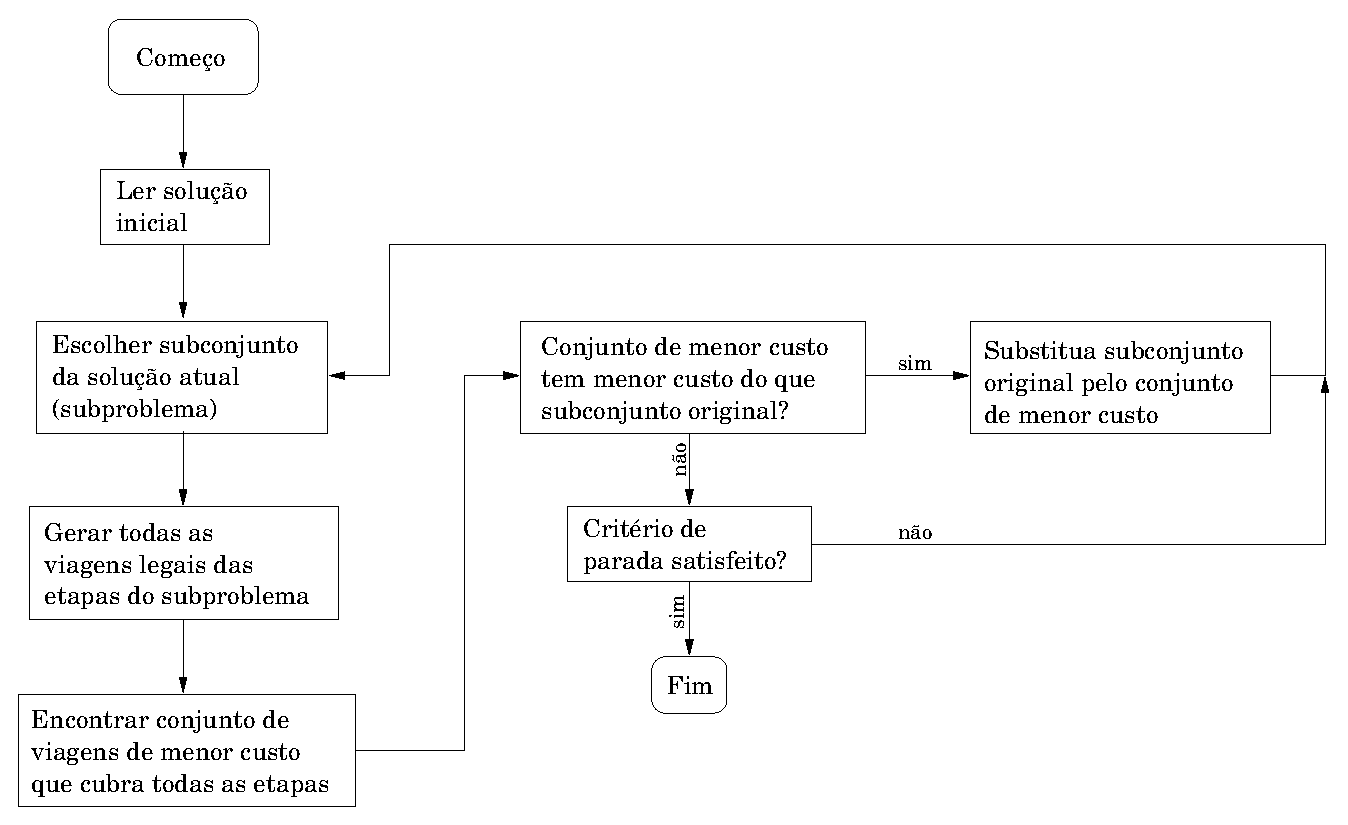
\includegraphics[scale=0.6]{fig/localsearch.eps}
		\caption{Algoritmo para o método da busca local. O fluxograma mostra como o processo de 
		otimização repete o loop de gerar viagens e encontrar um subconjunto ótimo otimizar até que
		algum critério de parada seja atingido.}
		\label{fig:busca_local}
	\end{center}
\end{figure}

A escolha do subproblema de forma aleatória é uma das mais simples possíveis. Algumas outras 
propostas foram consideradas~\cite{anbil91a,arabeyre69}. Entretanto, a escolha aleatória ainda
parece ser a que apresenta melhor custo-benefíficio. Assim, adotamos a estratégia aletória em nossa 
implementação.

%%%%%%%%%%%%%%%%%%%%%%%%%%%%%%%%%%%%%%%%%%%%%%%%%%%%%%%%%%%%%%%%%%%%%%%%%%%%%%%%%%%%%%%%%%%%%%%%%%%%

\section{Algoritmo Genético}
\label{sec:metodos_genetico}

Computação evolucionária tem se tornado um termo padrão para indicar técnicas de resolução de 
problemas que usam princípios de {\it design} inspirados a partir de modelos da evolução natural das
espécies.

Algoritmos genéticos~\cite{holland75, goldberg89} representam um tipo de estratégia desenvolvida
dentro da área de computação evolucionária. A abordagem comum dos algoritmos é baseada no uso de uma
população e de operadores inspiradas pela genética de seres vivos para explorar o espaço de busca
(os operadores mais típicos são {\it reprodução}, {\it mutação} e {\it recombinação}). Cada
indivíduo no algoritmo representa direta ou indiretamente (através de um esquema de decodificação)
uma solução para o problema em consideração. O operador de reprodução se refere ao processo de
seleção de indivíduos que irão sobreviver e se tornar parte da próxima geração. Esse operador
normalmente utiliza um viés em direção à indivíduos de boa qualidade: quanto melhor a função
objetivo de um indivíduo, maior será a probabilidade do indivíduo ser selecionado e se tornar membro
da próxima geração. O operador de recombinação (também chamado de {\it crossover}) combina partes de
dois ou mais indivíduos para gerar novos indivíduos, também chamados de {\it offspring}. O operador
de mutação é um operador unitário que introduz modificações aleatórias em um indivíduo. Algoritmos
genéticos tipicamente utilizam variáveis com valores binários ou discretos para representar
informação em seus indivíduos, priorizando o uso de recombinação.

O uso de técnicas evolucionárias aplicadas à resolução do problema {\it set cover} é encontrado
em~\cite{beasley95}. Inspirado nesse trabalho, os autores de~\cite{kornilakis02} propõem um
algoritmo genético para resolver o problema da determinação de viagens. Na verdade, o algoritmo
proposto em~\cite{kornilakis02} é uma especialização daquele em~\cite{beasley95}, com algumas
modificações que visam a minimização do número de {\it deadheads} na solução final e um método para
corrigir soluções que violam restriçoes (soluções que não cobrem todos as etapas). Estudamos os dois
trabalhos em detalhes. Vamos apresentar abaixo uma síntese de seus métodos e descrever a nossa
implementação.

Inicialmente um determinado conjunto de viagens é gerado. O processo de otimização do algoritmo
genético se refere a esse conjunto de viagens. Indivíduos são representados por cromossomos. Uma
codificação binária é utilizada para cada cromossomo. Cada gene corresponde a uma viagem e quando 
seu valor é 0, significa que aquela viagem não faz parte da solução. Se o valor for 1, então a 
viagem correspondente é incluída na solução.

A função objetivo utilizada para representar a qualidade ({\it fitness}) de cada indivíduo é
%
\begin{equation*}
	f = \sum_i c_i g_i + \rho D \ev
\end{equation*}
%
onde $c_i$ é o custo da $i$-ésima viagem, $g_i$ é o valor do $i$-ésimo gene, $\rho$ é uma
constante utilizada para penalizar etapas que são cobertas mais de uma vez e $D$ o número total de
tais etapas na solução.

A seleção dos membros da população que se tornarão pais é baseada em suas posições na população, as
quais são ordenadas em ordem decrescente com base no valor da função de {\it fitness} (método da
roleta). Ou seja, o indivíduo mais apto é o que vai ter maior chance de ser escolhido.

Para selecionar o indivíduo que será substituído a cada geração, escolhemos uniformemente dentre
todos aqueles que apresentam valor de {\it fitness} menor do que da média da população.

Uma vez que dois pais tenham sido escolhidos, a operação de {\it crossover} é aplicada de forma a
se obter um novo indivíduo que herde características de ambos os pais: se um gene tem o mesmo valor
no cromossomo dos dois pais, esse valor é atribuído ao mesmo gene do cromossomo filho. Se os valores
forem diferentes, o gene correspondente no {\it offspring} pode ser 0 ou 1, com igual probabilidade.
Isso define um operador de {\it crossover} uniforme.

A operação de mutação é aplicada ao indivíduo filho gerado. O objetivo da mutação é prevenir que a
busca fique presa em um mínimo local. Isso é feito alterando aleatóriamente alguns dos genes do
cromossomo gerado, de forma direcionar a busca em direção a novas áreas no espaço de busca. O número
de genes $\mu$ a serem mutados é dado pela fórmula~\cite{beasley95} ({\it steady-state replacement
model})
%
\begin{equation*}
\mu	= \left\lceil \frac{m_f}{1+\exp{\left(-4m_g(k - m_c)/m_f\right)}} \right\rceil \ev
\end{equation*}
%
onde $k$ é o número da geração, $m_f$ especifica a taxa de mutação estável final, $m_c$ representa o
número de gerações no qual a taxa $m_f/2$ é atingida e $m_g$ específica o gradiente em $k = m_c$. Os
parâmetros acima podem ser livremente escolhidos de modo a produzir os melhores resultados. Assim,
escolhendo $\mu$ genes do cromossomo aleatoriamente, cada um será mutado para 0 com probabilidade
igual ao número de zeros do cromossomo mais apto da população, de outra forma será mutado para 1.

Pode acontecer que depois das operações de {\it crossover} e mutação o cromossomo gerado não mais
represente uma solução viável, \ie, nem todas as etapas estão presentes em pelo menos uma das
viagens do cromossomo. Deve-se então aplicar um algoritmo correctivo no novo indivíduo. Esse
algoritmo funciona de forma heurística alterando o valor de alguns genes para 1, até que todos os
voos sejam cobertos, tornando a solução viável: para cada perna descoberta da solução, adicionamos
uma viagem que cobre aquela perna. Para isso, escolhemos uma viagem de baixo custo que quando
selecionada cubra o máximo de pernas descobertas possível e o mínimo de pernas já cobertas. Para
mais detalhes e uma descrição forma do método corretivo, consulte~\cite{beasley95}.

A população inicial criada pelo algoritmo deve ter a maior diversidade de indivíduos possível para
que uma boa parte do espaço de busca seja explorado no início. Para tanto, geramos os indivíduos
iniciais escolhendo viagens aleatoriamente, que não tenham pernas comuns com as outras viagens já
selecionadas. Quando atingirmos um ponto em que não é mais possível escolher tais viagens, rodamos o
algoritmo corretivo para tornar o cromossomo viável. Assim, bastante aleatoriedade estará presente
na geração dos indivíduos, de forma que a população criada apresentará a diversidade desejada.

A implementação do algoritmo genético descrito acima não se mostrou satisfatória. O problema está no
fato de precisarmos inicialmente gerar um conjunto com um grande número de viagens para serem
otimizadas, no primeiro passo do algoritmo. Para instâncias grandes esse número é muito grande,
tornando inclusive seu armazenamento em memória complicado. Mesmo utilizando estruturas de dados
mais inteligentes para armazenar informações como {\it hashes} e {\it lists}, o algoritmo torna-se
demasiadamente lento.

O essencial para o algoritmo, entretanto, é possuir pelo menos um conjunto de viagens que gere
alguma solução viável. Isso é fácil de ser obtido, conforme sugerimos no final da
Seção~\ref{sec:refatorando}, resultando em um conjunto relativamente pequeno de viagens. Todavia,
somente a partir desse conjunto, a geração dos indivíduos iniciais não apresentará a diversidade
necessária para uma exploração ampla do espaço de busca. Para contornar essa dificuldade, podemos
melhorar a qualidade de cada indivíduo iniciamente gerado aplicando o procedimento de busca local
descrito na seção anterior. Novas e melhores viagens serão geradas durante o procedimento,
aumentando a aptidão do indivíduo em construção. Essas viagens geradas são incluídas na construção
dos próximos indivíduos e estarão disponíveis para os operadores de {\it crossover}, mutação e para
o algoritmo corretivo. A ideia é semelhante é inspirada na heurística GRASP ({\it greedy randomized
adaptive search procedures})~\cite{feo89, feo95}.

Na Figura~\ref{fig:genetico} apresentamos uma descrição esquemática do algoritmo genético híbrido
implementado. O algoritmo é híbrido por que envolve alguns passos de otimização usando o 
procedimento de busca local para melhorar a qualidade e a diversidade da população inicial. Mais
epecificamnte, intrduzimos um parámetro $L$ que representa o número de iterações do tipo apresentado
na Figura~\ref{fig:busca_local} que um indivíduo deve se submeter antes de entrar na população 
inicial.

\begin{figure}[htbp]
	\begin{center}
		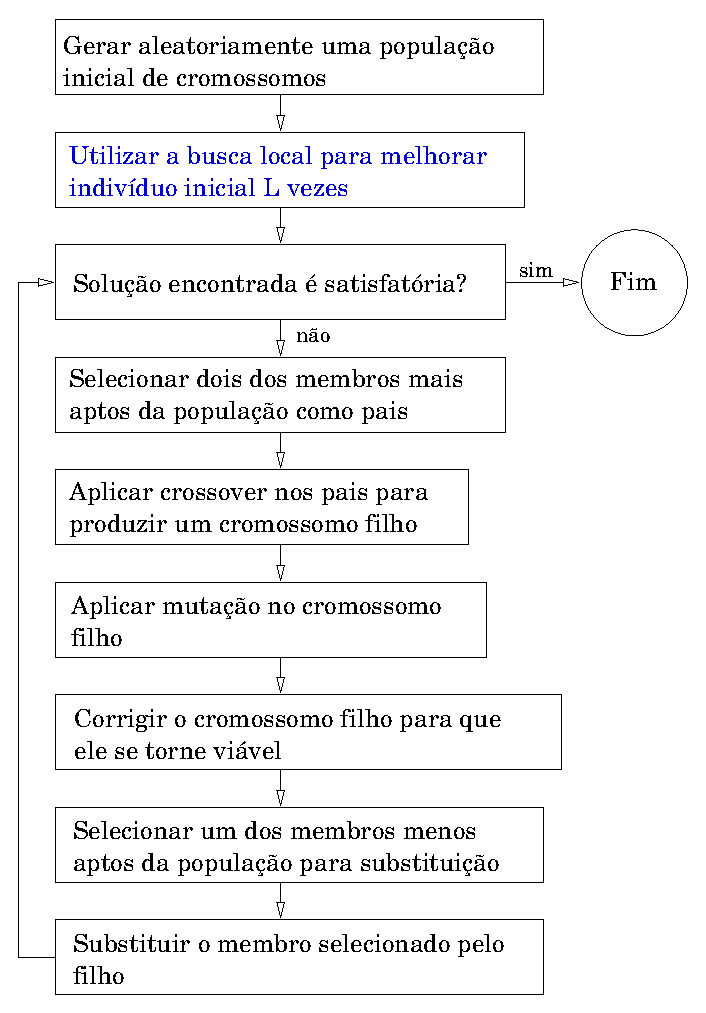
\includegraphics[scale=0.6]{fig/genetic.eps}
		\caption{Fluxograma mostrando o funcionamento do algoritmo genético híbrido proposto. O quadro 
		em azul representa uma novidade com relação ao algoritmo usual de~\cite{beasley95,kornilakis02},
		inspirado na heurística GRASP, resultando em um ganho considerável de qualidade e performance.}
		\label{fig:genetico}
	\end{center}
\end{figure}

%%%%%%%%%%%%%%%%%%%%%%%%%%%%%%%%%%%%%%%%%%%%%%%%%%%%%%%%%%%%%%%%%%%%%%%%%%%%%%%%%%%%%%%%%%%%%%%%%%%%

\section{Geração de Colunas}
\label{sec:metodos_colunas}

\begin{equation} \label{eq:sub}
	w^\ast = \min_{j = 1, \ldots, n} \left[ c_j - \sum_{i=1}^m \pi_i a_{ij} \right] \ev
\end{equation}

\begin{figure}[htbp]
	\begin{center}
		\includegraphics[scale=0.6]{fig/cg.eps}
		\caption{Fluxograma mostrando o funcionamento do procedimento de geração de colunas.
		O {\it princing problem} é traduzido em um problema de caminho mais curto com restrições.}
		\label{fig:cg}
	\end{center}
\end{figure}

\begin{figure}[htbp]
	\begin{center}
		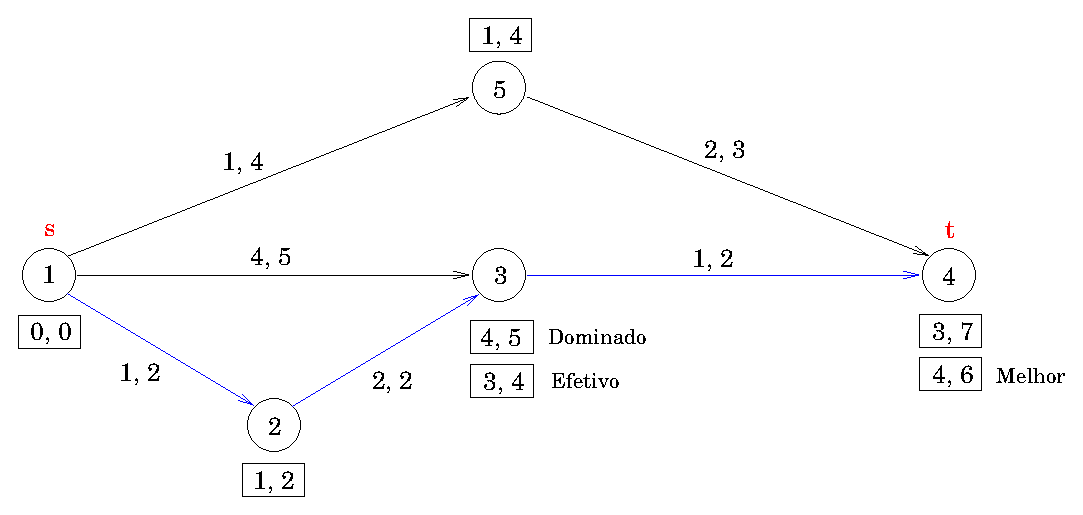
\includegraphics[scale=0.6]{fig/shortest_path.eps}
		\caption{Caminho mais curto com restrições entre os nós $s$ e $t$: $1 \to 2 \to 3 \to 4$.}
		\label{fig:shortest_path}
	\end{center}
\end{figure}

